% !TeX root = responsiveness_tr
% ================================================================
\section{Problem}\label{prresp_Problem}

\begin{figure*}
	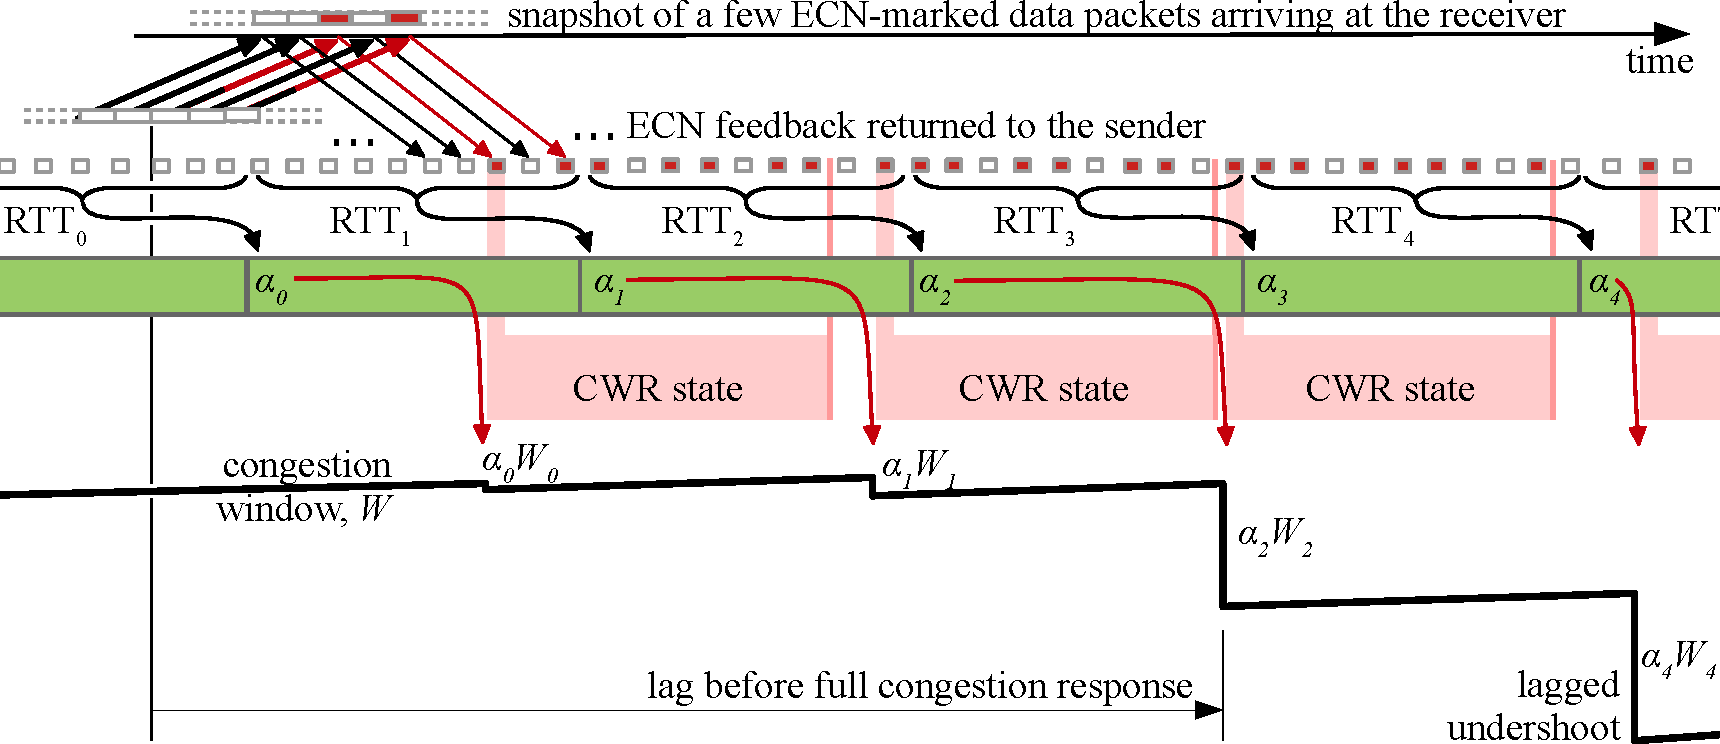
\includegraphics[width=\linewidth]{dctcp-feedback-lag}
	\caption{The problem: DCTCP's two stages for processing congestion feedback: 1)
	gathering feedback in a fixed sequence of rounds (RTT\(_i\)) to calculate the
	EWMA (\(\alpha_i\)); 2) applying this EWMA on the first feedback mark, when it
	has had no time to gather enough feedback, which leads to a typically
	inadequate congestion response before entering congestion window reduced (CWR)
	state, which suppresses any further response for a round. See text for full
	commentary.}
	\label{fig:dctcp-feedback-lag}
\end{figure*}

This report shows that common implementations of DCTCP~\cite{Alizadeh10:DCTCP} (e.g.\ in Windows,
Linux, or FreeBSD~\cite{Bensley17:DCTCP}) take up to two rounds before a change in
congestion on the path fully feeds into the moving average that regulates its
response. This is on top of the inherent round trip of delay in the feedback loop. 

A moving average intentionally dampens responsiveness so that there will only be a full response to a change if it sustains over the whole averaging period. However, the extra rounds we focus on here represent pure lag before that damping can even start. 

This means that established DCTCP flows take 2 or 3 rounds (rather than 1) before they even start to respond to a reduction in available capacity or yield to a new flow. In turn, this means that a new flow must either build up a large queue before any established flow yields, or it must enter the system very tentatively. Therefore, the algorithm in this report is at least part of a solution to the 'Prague Requirement' for 'faster convergence at flow start'~\cite[Appx A.2.3]{Briscoe15f:ecn-l4s-id_ID}.

Both extra rounds are due to DCTCP's two-stage process for responding to congestion (see \autoref{fig:dctcp-feedback-lag}). The
first stage introduces one round of delay (RTT\(_i\)) while it accumulates the
marking fraction before it can calculate the EWMA (\(\alpha_i\)). It
passes this to the second stage that reduces the congestion window
(\(W\)) by \(\alpha_i W_i\). The second extra round arises because the
second stage is triggered by congestion feedback (a red
ACK) that occurs independently of the regularly clocked first stage. 

So it takes two rounds before a full round of the congestion that triggered the
start of the second stage has fed through into the EWMA that the first stage
passes to the second. This is exacerbated by entering congestion window
reduced (CWR) state at the first sign of congestion,
which suppresses any further response for a round, just when more congestion
feedback is likely. Also, the lagged congestion response will tend to overrun into
the subsequent round, causing undershoot.

The problem seems to boil down to how to update the EWMA of marking on a per-ACK
basis. But, more specifically, the problem is how to keep the time
constant over which this per-ACK EWMA smooths itself to a set number of
rounds, even though the number of packets per round varies.

\section{Per-ACK EWMA}\label{prresp_Per-Packet_EWMA}

Instead of the EWMA of the marking probability being upscaled by a constant
factor, it is proposed to upscale it by \texttt{flight\_ / gain}, where
\texttt{flight\_} is the packets in flight, and \texttt{gain} is a constant
(\texttt{gain < 1}). Then, as shown below, the EWMA can be maintained by a
single continuous set of repetitive increments or decrements determined on each
ACK.

Although it updates every ACK, we show that scaling up the EWMA by
\texttt{flight\_} \emph{implicitly} smooths the EWMA over a characteristic
number of RTTs (specifically, \texttt{RTT/gain}), no matter how many ACKs there
are per RTT. This contrasts with \emph{explicitly} clocking per
round that requires the two-stage process with its inherent extra lag.

The scaled up EWMA is effectively a smoothed count of the number of congestion
marks per RTT, but scaled up by the constant \texttt{1/gain}. The number of
marks per RTT (\texttt{v}) is related to the marking probability (\texttt{p}) by
\texttt{v = p*flight\_}.

Classical congestion controls suppress any further response for a round because
their initial response is large and fixed. It seems wrong for DCTCP to mimic the
timing of a classical congestion response, when it does not mimic its size. On
first onset of congestion, DCTCP immediately responds with a tiny reduction
(based on the previous absence of congestion), but then perversely it suppress
any further response for a round trip.

So, once we have an EWMA of congestion marks that is updated continually on
every ACK, it becomes possible to spread the reduction over the round. Then,  if
congestion continues to rise during the round, the EWMA will grow, and the
response can pick up this growth as it proceeds.

\paragraph{Definitions of variables}
\begin{description}[nosep]
	\item [\texttt{G}] = \texttt{1/gain} (\(>1\)). By default in DCTCP \texttt{G = 16};
%	\item [\texttt{G\_shift}] = \texttt{lg(G)};
	\item [\texttt{av\_up}]: EWMA of the marks per round upscaled by \texttt{G};
	Alternatively, it might help to think of this as the EWMA of the marking
	probability (alpha in DCTCP) upscaled by \texttt{G * flight\_}. 
	\item [\texttt{flight\_}]: the number of packets in flight when the marking
	probablity was fed into the EWMA (used for explanation, but not in the code);
	\item [\texttt{flight}]: the number of packets in flight now;
	\item [\texttt{ce\_fb}] = 1 if ECN feedback per pkt; 0 otherwise.
\end{description}

\subsection{Intuition}\label{prresp_intuition}

In DCTCP, the EWMA, \texttt{alpha}, is maintained per round trip as follows (in
floating point arithmetic):
\begin{verbatim}
    alpha += (F - alpha)/G,
\end{verbatim}
where F is the fraction of marked bytes accumulated over the last round trip.

This can be approximated (see \autoref{prresp_approx}) by repeatedly updating
the EWMA on the feedback of every packet, but scaling down each update by the
number of packets in that round, \texttt{flight\_}. That is, the following
per-packet update:
\begin{verbatim}
    alpha += (ce_fb - alpha) / (flight_*G).
\end{verbatim}

The above per-packet update of the EWMA is roughly equivalent to the following
per-packet update of the upscaled EWMA, \texttt{av\_up}:
\begin{verbatim}
    av_up += ce_fb - av_up/(flight_*G).
\end{verbatim}

\subsection{Implementation}\label{prresp_implementation}

\subsubsection{Maintaining the EWMA}

The \texttt{ce\_fb} term can be implemented by adding 1 to \texttt{av\_up} on
feedback of each CE-marked packet. If \texttt{av\_up} was not upscaled by
\texttt{G}, this would equivalent to adding \texttt{1/G} of a mark.

The number of packets acknowledged in the current round is \texttt{flight}. So
repeatedly subtracting \texttt{av\_up/(flight\_*G)} on the arrival of every ACK
would reduce \texttt{av\_up} by \texttt{av\_up*flight/(flight\_*G)} in a round
(see \autoref{prresp_approx}). This approximates to \texttt{av\_up/G} per round.

\begin{verbatim}
On_each_ACK'd_packet {
  // Update EWMA
  av_carry = 
    div(av_carry.rem+av_up, flight*G);
  av_up += ce_fb - av_carry.quot;
}
\end{verbatim}

The pseudocode uses an integer division function \texttt{div()} with the same interface as \texttt{div()} in C's standard library.\footnote{\texttt{div()} can be thought of as a wrapper round \texttt{do\_div()}, which is intended for kernel use, but less readable for pseudocode.} Specifically, it returns both the quotient and the remainder in the following structure:
\begin{verbatim}
typedef struct {
  int quot;
  int rem;
} div_t;
\end{verbatim}
The variable \texttt{av\_carry} would be declared of type \texttt{div\_t}. It is used to carry forward the remainder to the invocation on the next ACK. The quotient will typically be either 0 or 1, which is then used to decrement the EWMA.

\autoref{fig:per-ack-ewma-verify} compares toy simulations of the above EWMA and
the DCTCP EWMA (without changing cwnd). It can be seen that, whenever marks
arrive, the algorithm always moves immediately, whereas DCTCP's EWMA does
nothing until the next round trip cycle.
\begin{figure}[h]
	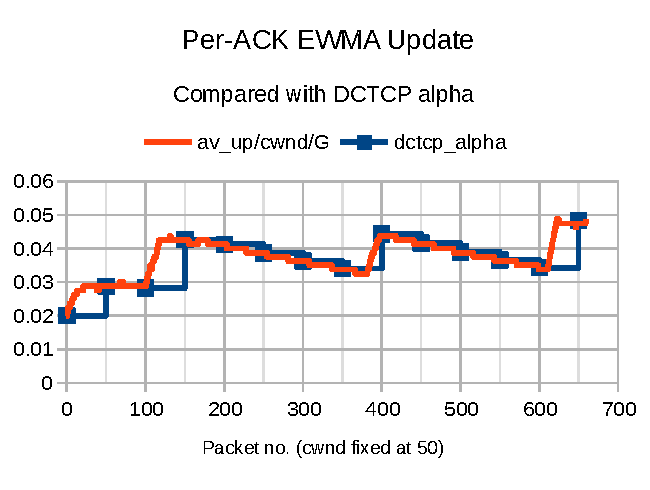
\includegraphics[width=\linewidth]{per-ack-ewma-verify}
	\caption{Initial verification of per-ACK EWMA algorithm (with constant \texttt{cwnd}).}\label{fig:per-ack-ewma-verify}
\end{figure}

\bob{Add discussion of initialization of the EWMA. To mimic DCTCP and Prague, on the first CE marked feedback, (av\_up = cwnd * G). However, it will be interesting to see whether we can improve on this in a further set of experiments; for instance using (av\_up = flight * G) instead}

\subsubsection{Responding to Congestion}\label{prresp_congestion_response}

The approach proposed in this section is not necessarily the final word on how
to use the per-ACK EWMA for scalable congestion control (see
\S\,\ref{prresp_future} for further ideas). Nonetheless, as a first step, we
build incrementally on DCTCP, using its teaching selectively, but not departing
too far from its intent. 

DCTCP reduces \texttt{cwnd} by \texttt{alpha*cwnd/2} in any round trip in which
CE feedback is present. The proposed approach reduces \texttt{cwnd} by half the
average number of marked packets per round, or \texttt{av\_up / (2*G)}. This is
broadly equivalent to DCTCP in that it maintains the scalable '\(1/p\)' response
function, except the following two slight differences could potentially alter
the steady-state outcome:
\begin{itemize}[nosep]
	\item The window reduction is taken as a proportion of what the window has been
	in recent rounds, not what it is now (as in DCTCP) (see
	\S\,\ref{prresp_Non-Concerns}).
	\item The window reduction is taken as a proportion of the amount of the window
	that has been \emph{used} in recent rounds, not the maximum that the flow was
	entitled to use, i.e.\ packets in flight not \texttt{cwnd}. Thus, if an
	application-limited flow has only used a quarter of the available window in
	recent rounds, the proposed reduction of \texttt{cwnd} will be only a quarter of
	that applied by DCTCP (see \S\,\ref{prresp_Advantage_App-Limited}).
\end{itemize}

The main departure from DCTCP is in the speed of response. Rather than reduce 
\texttt{cwnd} on the first sign of CE feedback then suppress further response
for a round trip, it is proposed to spread the reduction over the round
following the first sign of CE feedback. In other words, use the whole round
while in CWR state to reduce \texttt{cwnd} as the EWMA updates, such that, by
the end of the round it will still have reduced as much as it would have done if
the whole reduction had been applied at the end. 

This will exploit the fact that the EWMA (\texttt{av\_up}) is continually
updated on every ACK. So, at one extreme, if the first CE mark is immediately
followed by many others, the EWMA will rapidly increase early in the round of
CWR, and \texttt{cwnd} can be rapidly decreased accordingly. While, at the other
extreme, if the first CE mark is the only CE mark in the round, \texttt{cwnd}
will still have reduced by \texttt{alpha*cwnd/2} by the end of the round, but
the EWMA will hardly have increased above the value it took when the CWR round
started. 

To spread the reduction over the round, the proposed algorithm below does not
divide the round into an arbitrary number of points where \texttt{cwnd} is
altered by varying amounts. Instead, it decrements \texttt{cwnd} as soon as the
algorithm first calculates that at least one packet of movement is possible. 

\begin{verbatim}
On_each_ACK'd_packet {
  // Update EWMA
  av_carry = 
    div(av_carry.rem+av_up, flight*G);
  av_up += ce_fb - av_carry.quot;

  if (!cwr && ce_fb) {
    // Record start of CWR state
    next_seq = snd_next;
    cwr = true;
  }
  if (cwr) {
    // Check still in CWR round
    if (snd_una < next_seq) {
      // Multiplicative Decrease
      cwnd_carry = div(cwnd_carry.rem 
                   + av_up, flight*G*2);
      cwnd -= cwnd_carry.quot;
    } else {
      cwr = false;
    }
  }
}
\end{verbatim}

As in DCTCP, the EWMA is calculated continuously, but it is only used if there
is actual congestion marking, when it is applied for one round of CWR. %This is
%also similar to the approach used to smooth queue measurement in many classical
%AQMs (e.g.\ PIE, CoDel), where a control law continuously calculates a smoothed
%likelihood of signalling (drops or marks), but the AQM only emits signals if
%the actual queue is above a certain threshold, even though it continues to
%evolve the signalling level.

CWR state then takes on a meaning that is nearly the opposite of its classical
meaning. It no longer means `congestion window reduced; no further reduction for
a round'. Instead it means `congestion window \emph{reduction} in progress
during this round'. 

Although the motivation for this algorithm was not to prevent the stall caused
by sudden decrease in \texttt{cwnd}, it would probably serve to address this
problem as well. Therefore it should supplant proportional rate reduction
(PRR~\cite{IETF_RFC6937:PRR}), at least when responding to ECN.

Details of \texttt{cwnd} processing are omitted from the pseudocode if they are
peripheral to the proposed changes. For instance, in real code \texttt{cwnd}
would be prevented from falling below a minimum (default 2 segments), and the
slow-start threshold would track reductions in \texttt{cwnd} (but see
\S\,\ref{prresp_future} for alternative ideas). Also, the code would have to
handle acknowledgement of multiple packets at a time (potentially with different
congestion markings). It might also handle ECN markings on packets of different
sizes, but the Linux implementation of DCTCP works well enough without attending
to this degree of detail.

Also, for clarity, various integer arithmetic tricks are omitted from the
pseudocode, such as choosing a value of \texttt{G} that is a power of 2, so that
multiplication by \texttt{G} can be implemented with a bit-shift.

The pseudocode does, nonetheless, inherently attend to details such as loss of
precision due to integer truncation. And note that \texttt{cwnd} is not updated
on the ACK that ends CWR state, because it is updated on the marked ACK that
starts CWR state.

\subsubsection{The Whole AIMD Algorithm}\label{prresp_AIMD}

For completeness, the pseudocode below %in \autoref{fig:prresp_per-ack-aimd} 
includes a Reno-like additive increase.
This is intended for periods when the congestion control is close to its
operating point (if it is not, see \S\,\ref{prresp_future}).

%\begin{figure}[t]
\begin{verbatim}
On_each_ACK'd_packet {
  // Update EWMA
  av_carry = 
    div(av_carry.rem+av_up, flight*G);
  av_up += ce_fb - av_carry.quot;

  if (!ce_fb) {
    // Additive Increase
    cwnd_carry = 
      div(cwnd_carry.rem+G*2, flight*G*2);
    cwnd += cwnd_carry.quot;
  } else if (!cwr) {
    // Record start of CWR state
    next_seq = snd_next;
    cwr = true;
  }

  if (cwr) {
    // Check still in CWR round
    if (snd_una < next_seq) {
      // Multiplicative Decrease
      _denom = flight*G*2;
      cwnd_carry.rem = 
        _denom - cwnd_carry.rem;
      cwnd_carry = 
        div(cwnd_carry.rem+av_up, _denom);
      cwnd_carry.rem = 
        _denom - cwnd_carry.rem;
      cwnd -= cwnd_carry.quot;
    } else {
      cwr = false;
    }
  }
}
\end{verbatim}
%\caption{The whole per-ACK AIMD algorithm}
%\label{fig:prresp_per-ack-aimd}
%\end{figure}

Unlike DCTCP, the proposed algorithm does not suspend additive increase during
CWR state, with the following reasoning. DCTCP-like congestion controls are
designed to induce roughly 2 ECN marks per round trip in steady state, so RTTs
without marks are not meant to happen. Confining increase to periods that are
not meant to happen creates an internal conflict within DCTCP's own design.
Then, the algorithm's only escape is to store up enough decrease rounds to make
space for a compensating period of increase. This has been found to cause
unnecessary queue variation.

Instead, we continue additive increase regardless of CWR state. In place of
suspending additive increase for a whole round, a fractional increase is
calculated per-ACK (as in most TCP implementations) but it is skipped if an ACK
carries congestion feedback. This thins down the additive increase as congestion
rises (see \S\,3.1 of \cite{Briscoe17a:CC_Tensions_TR}).

Also unlike DCTCP, the proposed algorithm increases \texttt{cwnd} by one segment
over the actual window of packets in flight, not over the congestion window
(which might not be fully used).

The additive increase stores its remainder in the same \texttt{*cwnd\_carry}
variable as the multiplicative decrease. So both numerator and denominator are
scaled up such that AI uses the same denominator parameter as MD, otherwise the
upscaling of the carry variable would be different.

Naively, the remainder could be added for AI and subtracted for MD. Instead, it is always added, but before and after the MD, it is respectively flipped to the opposite end of the number space of the denominator and back again. Whichever direction cwnd last moved in, this ensures that the remainder always lies in the range [0,\texttt{\_denom}-1].
This is preferable to handling a negative carry, which would halve the number
space available for the scaled up variables.

\section{(Non-)Concerns}\label{prresp_Non-Concerns}

\subsection{Circular Dependency?}\label{prresp_No_Circular_Dependency}

There seems to be a circular dependency, because \texttt{av\_up} is both
upscaled by \texttt{flight\_} then used to update \texttt{cwnd}, which
determines \texttt{flight}.

In fact, \texttt{av\_up} is upscaled by \texttt{flight\_} (note the trailing
underscore), which is what \texttt{flight} \emph{was} at the time of each
repetitive decrement or increment of \texttt{av\_up}. So \texttt{av\_up} depends
on an implicit exponentially weighted moving average of \texttt{flight} with a
characteristic smoothing timescale of \texttt{G} round trips. This removes any
circular dependency.

\subsection{Advantage to Application Limited
	Flows?}\label{prresp_Advantage_App-Limited}

The reduction to \texttt{cwnd} is spread over the \texttt{flight} packets in a
round of CWR, so each reduction is scaled down by \texttt{flight} in the
denominator of the call to \texttt{div()}. This means that the
decrease of \texttt{cwnd} is actually by a multiplicative factor of
\texttt{flight}, not of \texttt{cwnd}.

If a flow is not application-limited, the two amount to the same thing. But for
app-limited flows, \texttt{flight} can be lower than \texttt{cwnd}, so the
reduction in \texttt{cwnd} will be lower.

If a flow is only using a fraction of its congestion window, but it is still
experiencing congestion, there is an implication that other flow(s) must have
filled the capacity that the app-limited flow is `entitled' to but not using.
Then, it could be argued that the other flows have a higher \texttt{cwnd} than
they are `entitled' to, so that the app-limited flow can reduce its
`entitlement' (\texttt{cwnd}) less than these other flows in response to
congestion.

If this argument is not convincing, the reduction in \texttt{cwnd} could be
scaled up by \texttt{cwnd/flight}. However, it is believed that the code is
reasonable, perhaps better, as it stands.

Similar arguments can be used to motivate additive increase over the actual
number of packets in flight, rather than the potential congestion window.

\section{Evaluation Plan}\label{prresp_Evaluation}

For research purposes, we ought not to introduce two changes at once, without
evaluating each separately. Therefore, initially, we ought to use the
continually updated EWMA, \texttt{av\_up} to reduce \texttt{cwnd} in the
classical way. That is, on the first feedback of a CE mark, reduce \texttt{cwnd}
once by \texttt{av\_up/(2*G)}. Then suppress further response for a round (CWR
state). This should remove one round of lag (originally spent accumulating the
marking fraction), but not the rest (spent reducing cwnd in response to a single
mark, then doing nothing for a round while the extent of marking is becoming
apparent).

Initial experiments will need to compare how quickly a DCTCP flow in congestion
avoidance can reduce in response to a newly arriving flow or a reduction in
capacity.

The Prague reference implementation should be used as the baseline, given it is
probably the best possible implementation of a per-RTT EWMA.%
%
\footnote{'Bugs' in the implementation of the EWMA in DCTCP have been fixed in
	TCP Prague, which raises the question of which variant of the EWMA code should
	be used as the baseline to compare with. Prior to a 2015
	patch~\cite{shewmaker15:Linux_DCTCP_EWMA}, the integer arithmetic for the EWMA
	in Linux floored at 15/1024, which ensured a minimum window reduction even after
	an extended period without congestion marking. That patch toggled the EWMA to
	zero whenever it tried to reduce \texttt{alpha} below that floor, and remained
	unresponsive until congestion was sufficient to toggle \texttt{alpha} back up to
	16/1024. The TCP Prague reference implementation maintains the EWMA in an
	upscaled variant of \texttt{alpha}, as well as using higher precision and
	removing rounding bias.}%
%
But it might also be interesting to compare this with the pre-2019
implementation of DCTCP that might have accidentally been more responsive in
many scenarios. This would be possible Without winding all the code back to that
date by simply setting a floor for \texttt{alpha} at 15/1024 in the Prague code.

Pacing should be enabled in both A and B tests. But, initially, segmentation
offload should be disabled, to simplify interpretation of the results, before
enabling offload in both A and B tests together.

Initially the same gain as DCTCP (1/16) ought to be used. But it is possible
that the reason DCTCP's gain had to be so low was because of the two rounds of
built in lag in the algorithm. Therefore, it will be interesting to see if the
gain can be increased (from 1/16 to 1/8 or perhaps even 1/2 ought to be tried).

The thinking here is that a fixed amount of lag in a response is not the same as
smoothing. Lag applies the same response but later. Smoothing spreads the
response out, adding lag to the end of the response, but not to the start. Given
every DCTCP flow's response to each change has been lagged by 2 rounds, it is
possible that all flows have had to be smoothed more than necessary, in order to
prevent the excessively lagged responses from causing over-reactions and
oscillations.

Our motivation for improving DCTCP's responsiveness is to ensure established
flows yield quickly when new flows are trying to enter the system, without
having to build a queue. However, removing up to two rounds of unnecessary lag
should also help to address the incast problem, at least for transfers that last
longer than one round. Therefore, incast experiments could also be of interest.

It will also be necessary to check performance in the following cases that might
expose poor approximations in the algorithm (relative to DCTCP):
\begin{enumerate}
	\item When the packets in flight has been growing for some time;
	\item \ldots{}or shrinking for some time;
	\item When the flow is application limited, with packets in flight varying
	wildly, rather than tracking the smoother evolution of \texttt{cwnd}.
\end{enumerate}

\bob{Outcome of the evaluations to be added here.}

\section{Related Work}\label{prresp_related}
\balance
Reducing \texttt{cwnd} in one RTT by half of the marks per round trip
(\texttt{av\_up/2/G}) is similar but not the same as Relentless
TCP~\cite{Mathis09:Relentless}, which reduces \texttt{cwnd} by half a segment on
feedback of each CE-marked packet. The difference is that \texttt{av\_up} is a
moving average, so it does not depend on the number of marks in any specific
round, whereas the Relentless approach does. Relentless was designed for the
classical approach with smoothing in the network, so it immediately applies a
full congestion response without smoothing. In contrast, using the moving
average implements the smoothing in the sender.

Like DCTCP, the per-ACK congestion response proposed in section 5.2 of
\cite{Alizadeh11:DCTCP_Analysis} maintains an EWMA of congestion marking
probability, \texttt{alpha}. But, unlike DCTCP, it reduces \texttt{cwnd} by half
of \texttt{alpha} (in units of packets) on feedback of each ECN mark. This is
partway between Relentless and DCTCP, because it uses the smoothed average of
marking, but it applies it more often in rounds with more marks. This still
causes considerable jumpiness, because marks tend to be bunched into one round
then clear for a few rounds, particularly with step-marking. In contrast, the
approach proposed in the present paper limits the reduction within any one round
to the averaged number of marks per round (as DCTCP itself does). %Nonetheless,
%it removes the round of lag that DCTCP's EWMA uses to accumulate the marking
%probability, and it spreads the reduction over a round to ensure that it picks
%up feedback as soon as it arrives.

\section{Ideas for Future Work}\label{prresp_future}

An EWMA of a queue-dependent signal is analogous to an integral controller. It
filters out rapid variations in the queue that do not persist, but it also
delays any response to variations that do persist. Faster control of dynamics
should be possible by adding a proportional element, to create a
proportional-integral (PI) controller within the sender's congestion control.
The proportional element would augment any reduction to the congestion window
dependent on the rate of increase in \texttt{av\_up}.

Separately, it would be possible to use the per-ACK EWMA of marks per round
(\texttt{av\_up}) as a good indicator of whether a flow has lost its closed-loop
control signal, for instance because another flow has left the bottleneck, or
capacity has suddenly increased. A flow could then switch into a mode where it
searches more widely for a new operating point, for instance using paced
chirping~\cite[\S\,3]{Misund19a:Paced_Chirping_Linux}. To deem that the closed
loop signal had significantly slowed, it might calculate the average distance
between marks implied by the EWMA \texttt{av\_up}, multiply this by a heuristic
factor, then compare this with the number of packets since the last mark.
Alternatively, it might detect when the EWMA of the marks per round had reduced
below some absolute threshold (by definition, the marks per round of a scalable
congestion control in steady state should be invariant for any flow rate).
